\documentclass[9pt,a4paper,final]{article}
\setlength{\textwidth}{450pt}
\setlength{\oddsidemargin}{0pt}
%----------------------------------------------------------------------
\usepackage[dvipdfmx]{graphicx}
\usepackage{amsmath}
\usepackage{amsfonts}
\usepackage{amsthm}
\usepackage{comment}
\usepackage{pgfplots}
\usepackage{mathtools}
\mathtoolsset{showonlyrefs}
%-----------tikz--------------------------------------------------------
\usepackage{tikz}
\usetikzlibrary{positioning}
\usetikzlibrary{arrows}
%-----------newcommand--------------------------------------------------
\begin{document}


\pgfplotsset{width=5cm}
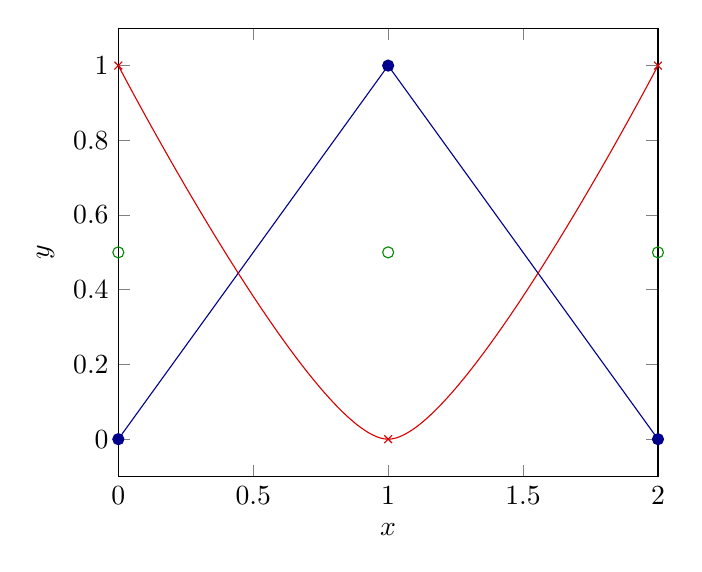
\begin{tikzpicture}
\begin{axis}[compat=1.17,xlabel={$x$},ylabel={$y$},enlarge x limits=false]
\addplot[blue!55!black,mark=*] coordinates{(0,0)(1,1)(2,0)};
\addplot[red!85!black,smooth,mark=x] coordinates{(0,1)(1,0)(2,1)};
\addplot[green!55!black,mark=o,only marks] coordinates{(0,0.5)(1,0.5)(2,0.5)};
\end{axis}
\end{tikzpicture}


%\pgfplotsset{width=5cm}
%\begin{tikzpicture}[remember picture]
%\begin{axis}[compat = newest,xlabel={$x$},ylabel={$y$}]
%\addplot[red,smooth] table[x=x,y=y] {data/vrol0.dat};
%\addplot[red,only marks,mark = |] table[x=x,y=c] {data/vrol0xyd.dat};
%\addplot[blue,smooth,dashed] table {data/vrol0xyexact.dat};
%\end{axis}
%\end{tikzpicture}
%
%
%\pgfplotsset{width=7cm}
%\begin{tikzpicture}[remember picture]
%\begin{axis}[compat = newest,xlabel={$t$},ylabel={Error},xmin=0,xmax=40,ymin=0]
%\addplot[smooth] table[x expr =\coordindex*0.1, y index = 0] {data/errorol.dat};
%\addlegendentry{$\Delta t=0.1, \Delta s = 0.2$} % 4.8 * 10^2 sec
%\addplot[smooth,dashed] table[x expr =\coordindex*0.05, y index = 0] {data/eol005.dat};
%\addlegendentry{$\Delta t=0.05, \Delta s = 0.2$} % 9.6 * 10^2 sec 
%\addplot[smooth,densely dotted] table[x expr =\coordindex*0.1, y index = 0] {data/eols.dat};
%\addlegendentry{$\Delta t=0.1, \Delta s = 0.1$} % 3.6 * 10^3 sec
%\end{axis}
%\end{tikzpicture}

\end{document}
